% Template LaTeX source file for homework problem solutions.
% Alan T. Sherman (9/9/98)

% Running LaTeX
%
% Name this file FOO.tex
% latex FOO
% latex FOO   
%    (You have to run latex twice to get the cross references correct.
%     Running latex creates a file FOO.dvi 
%     You can view dvi files with the program xdvi )
% xdvi FOO.dvi &
%
% lpr -d FOO.dvi
%    (To print the dvi file.   Be sure to use the "-d" print option,
%     and be sure your printer can handle dvi files (not all printers can).
%     Do NOT print with "lpr FOO.dvi", which will print tens of pages
%     of unreadable dvi source code. Printing a postscript (ps) file
%     is usually more reliable, as explained below.)
%
% dvips FOO.dvi
%    (To create a postscript file named FOO.ps 
%     which you can view with the program ghostview )
% ghostview FOO.ps &
% lpr FOO.ps
%    (To print the ps file.)

%%%%%%%%%%%%%%%%%%%%%%%%%%%%%%%%%%%%%%%%%%%%%%%%%%%%%%%%%%%%%%%%%%%%%%

\documentclass[12pt]{article}
\usepackage{amsmath,amssymb}
\usepackage[framed,numbered,autolinebreaks,useliterate]{mcode}
\usepackage{graphicx}
\usepackage[justification=centering]{caption}
\usepackage{float}

% Set the margins
%
\setlength{\textheight}{8.5in}
\setlength{\headheight}{.25in}
\setlength{\headsep}{.25in}
\setlength{\topmargin}{0in}
\setlength{\textwidth}{6.5in}
\setlength{\oddsidemargin}{0in}
\setlength{\evensidemargin}{0in}




%%%%%%%%%%%%%%%%%%%%%%%%%%%%%%%%%%%%%%%%%%%%%%%%%%%%%%%%%%%%%%%%%%%%%%%
% Macros

% Math Macros.  It would be better to use the AMS LaTeX package,
% including the Bbb fonts, but I'm showing how to get by with the most
% primitive version of LaTeX.  I follow the naming convention to begin
% user-defined macro and variable names with the prefix "my" to make it
% easier to distiguish user-defined macros from LaTeX commands.
%
\newcommand{\myN}{\hbox{N\hspace*{-.9em}I\hspace*{.4em}}}
\newcommand{\myZ}{\hbox{Z}^+}
\newcommand{\myR}{\hbox{R}}

\newcommand{\myfunction}[3]
{${#1} : {#2} \rightarrow {#3}$ }

\newcommand{\myzrfunction}[1]
{\myfunction{#1}{{\myZ}}{{\myR}}}


% Formating Macros
%

\newcommand{\myheader}[4]
{\vspace*{-0.5in}
\noindent
{#1} \hfill {#3}

\noindent
{#2} \hfill {#4}

\noindent
\rule[8pt]{\textwidth}{1pt}

\vspace{1ex} 
}  % end \myheader 

\newcommand{\myalgsheader}[0]
{\myheader{METU, Computer Engineering}
{CENG780 - Sparse Matrix Computations Homework {\bf 4} by {\bf Berkay Şahin}  - \bf 2232668} {Spring 2022}{}}

% Running head (goes at top of each page, beginning with page 2.
% Must precede by \pagestyle{myheadings}.
\newcommand{\myrunninghead}[2]
{\markright{{\it {#1}, {#2}}}}




%%%%%% Begin document with header and title %%%%%%%%%%%%%%%%%%%%%%%%%

\begin{document}

\myalgsheader
\pagenumbering{gobble}
\pagestyle{plain} 

\section{Introduction} 
\quad This report's focus is on eigenvalue and eigenvector (eigenpair) problems of a coefficient matrix. 
\[A*x = \lambda*x\] 
\quad We have power methods, for finding the largest (or the smallest with inverse option) eigenpairs. These methods can only handle one eigenpair. However, there are also simultaneous subspace iterations methods for finding eigenpairs till k-th order.\\ \\
$\bullet$ The Plain Simultaneous Subspace Iterations (SSI) \\ 
$\bullet$ Simultaneous Inverse Subspace Iterations (SII)\\ \par
SSI is used for finding the largest eigen pairs, on the other hand, SII is used for the smallest eigenpairs. The MATLAB code plots the timing measurements of these methods, besides MATLAB built-in eigs() function result. Test matrices are "LUND A", "BFW62 B", and "PLAT362".

\section{Implementation} 

\begin{lstlisting}
clear all;
close all;
A = mmread('inputs/plat362.mtx');

%% parameters
k = 1;
X = ones(length(A), k);
max_iter = 100000;
tol = 1e-12;

%% matlab eigs functions for finding largest and smallest eigenpairs
tic;
[V1, D1] = eigs(A, [], k, 'largestabs');
eigs_max_time = toc;
V1 = abs(V1);
tic;
[V2, D2] = eigs(A, [], k, 'smallestabs');
V2 = abs(V2);
eigs_min_time = toc;

%% ssi(subspace iterations) and sii(subspace inverse iterations) algorithms
i = 0;
tic;
while (i < max_iter) & tol < norm(abs(V1) - abs(X))
Z = A*X;
[X, R] = qr(Z, 0);
i = i+1;
end
iteration_ssi = i;
ssivec = abs(X);
for i = 1:k
ssival_(:, 1) = A * X(:, i);
ssival(i,i) = ssival_(1, 1) / X(1, i);
end
ssi_time = toc;

X = ones(length(A), k);
i = 0;
tic;
A = inv(A);
while (i < max_iter) & tol < norm(abs(V2) - abs(X))
Z = A*X;
[X, R] = qr(Z, 0);
i = i+1;
end
iteration_sii = i;
siivec = abs(X);
for i = 1:k
siival_(:, 1) = A * X(:, i);
siival(i,i) = 1 / (siival_(1, 1) / X(1, i));
end
sii_time = toc;

%% figures
xa = categorical({'eigs()_l_a_r_g_e_s_t Time Spent','SSI Time Spent','eigs()_s_m_a_l_l_e_s_t Time Spent','SII Time Spent'});
xa = reordercats(xa, {'eigs()_l_a_r_g_e_s_t Time Spent','SSI Time Spent','eigs()_s_m_a_l_l_e_s_t Time Spent','SII Time Spent'});
ya = [eigs_max_time, ssi_time, eigs_min_time, sii_time];
b = bar(xa,ya, 0.1);
xtips1 = b(1).XEndPoints;
ytips1 = b(1).YEndPoints;
labels1 = string(b(1).YData);
text(xtips1,ytips1,labels1,'HorizontalAlignment','center',...
'VerticalAlignment','bottom')
title('Time Consumption Comparison');
subtitle('Built-in eigs() with SSI and SII, tolerance value is 1e-12');
ylabel('Time (sec)')
ylim([0, max(ya)+max(ya)/10])
grid minor











\end{lstlisting} 
\centering Main code including all algorithms \break \break


\raggedright \quad Firstly parameters are set. Then, eigs() function are run with recording time for two of the methods. Then implemented algorithms are run with recording time. At the result, some eigenvector components are resulted in negative sign as regards to eigs() results. Therefore; abs() function is called for eigenvectors. At the and, plotting functions take part.  \\[0.75in]

\begingroup

\fontsize{16pt}{12pt}\selectfont
\centering \textbf{Computing Platform}

\endgroup

\raggedright

\hspace{1cm}

\quad \textbf{Processor:} 11th Gen Intel(R) Core(TM) i7-11800H @ 2.30GHz   2.30 GHz \\
\quad \textbf{RAM:} 16.0 GB (15.7 GB usable) \\
\quad \textbf{OS:} Windows 11 Home \\
\quad \textbf{Software:} MATLAB R2021b\\
\quad \textbf{version -blas:} Intel(R) Math Kernel Library Version 2019.0.3 Product Build 20190125 for Intel(R) 64 architecture applications, CNR branch AVX512\_E1 \\
\quad \textbf{version -lapack:} Intel(R) Math Kernel Library Version 2019.0.3 Product Build 20190125 for Intel(R) 64 architecture applications, CNR branch AVX512\_E1, supporting Linear Algebra PACKage (LAPACK 3.7.0) \\[0.75in]

\begingroup

\fontsize{16pt}{12pt}\selectfont
	\centering \textbf{Test Matrices}

\endgroup

\begin{figure}[h]
	\centerline{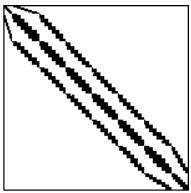
\includegraphics[scale=.7]{lunda.jpg}}
	\caption{\textbf{LUND A, Original Harwell sparse matrix test collection} \\ 147 x 147, 1298 entries}
	\label{fig1}
\end{figure}


\begin{figure}[h]
	\centerline{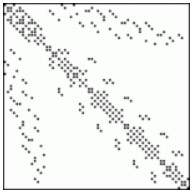
\includegraphics[scale=.7]{bfw.jpg}}
	\caption{\textbf{BFW62B, Bounded Finline Dielectric Waveguide} \\
	62 x 62, 342 entries}
	\label{fig2}
\end{figure}


\begin{figure}[h]
	\centerline{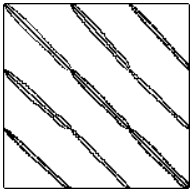
\includegraphics[scale=.7]{plat.jpg}}
	\caption{\textbf{PLAT362, Platzman's oceanographic models
			North Atlantic submodel} \\
	362 x 362, 3074 entries}
	\label{fig3}
\end{figure}


\section{Results} 

\begin{figure}[H]
	\centerline{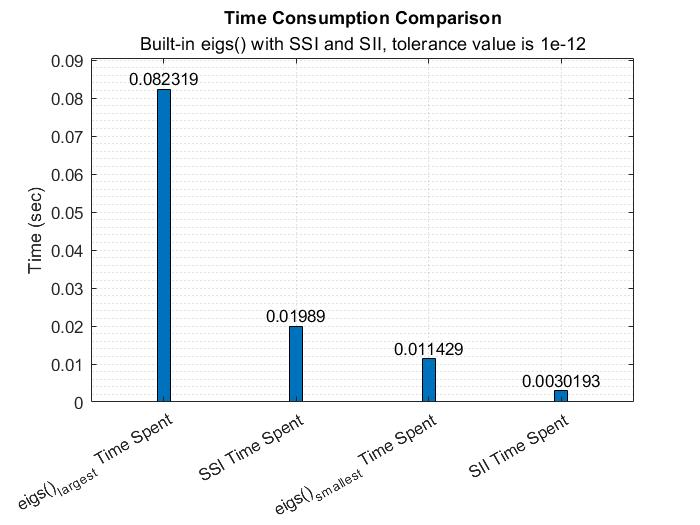
\includegraphics[height=9cm, width=12cm]{plot1lunda.jpg}}
	\caption{\textbf{LUND A, k = 1} \\ Iteration Number for SSI = 1687, Iteration Number for SII = 9}
	\label{fig4}\end{figure}

\begin{figure}[H]
	\centerline{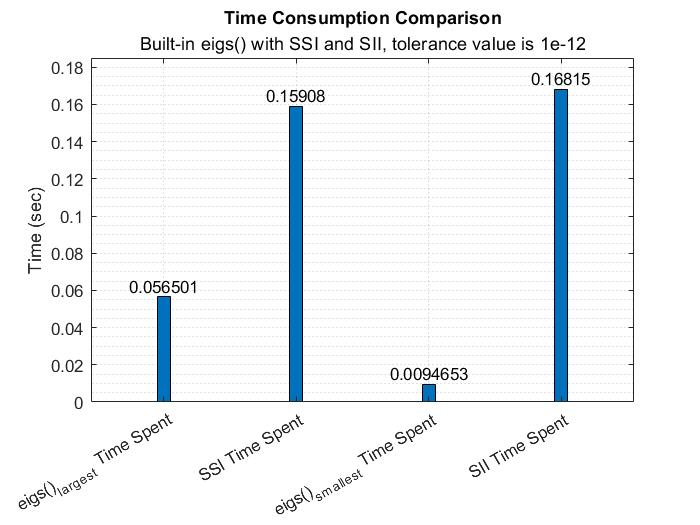
\includegraphics[height=9cm, width=12cm]{plot3lunda.jpg}}
	\caption{\textbf{LUND A, k = 3} \\ Iteration Number for SSI = 5041, Iteration Number for SII = 2833}
	\label{fig5}
\end{figure}

\begin{figure}[H]
	\centerline{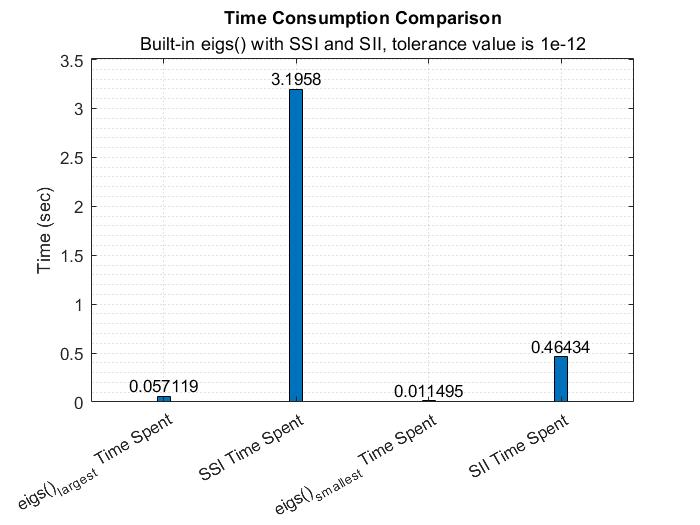
\includegraphics[height=9cm, width=12cm]{plot10lunda.jpg}}
	\caption{\textbf{LUND A, k = 10} \\ Iteration Number for SSI = 34269, Iteration Number for SII = 2834}
	\label{fig6}
\end{figure}

\begin{figure}[H]
	\centerline{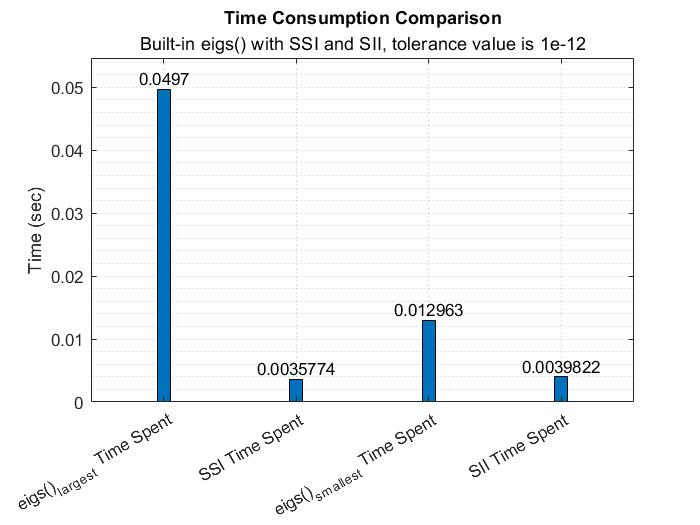
\includegraphics[height=9cm, width=12cm]{plot1bfw.jpg}}
	\caption{\textbf{BFW62B, k = 1} \\ Iteration Number for SSI = 1149, Iteration Number for SII = 905}
	\label{fig7}\end{figure}

\begin{figure}[H]
	\centerline{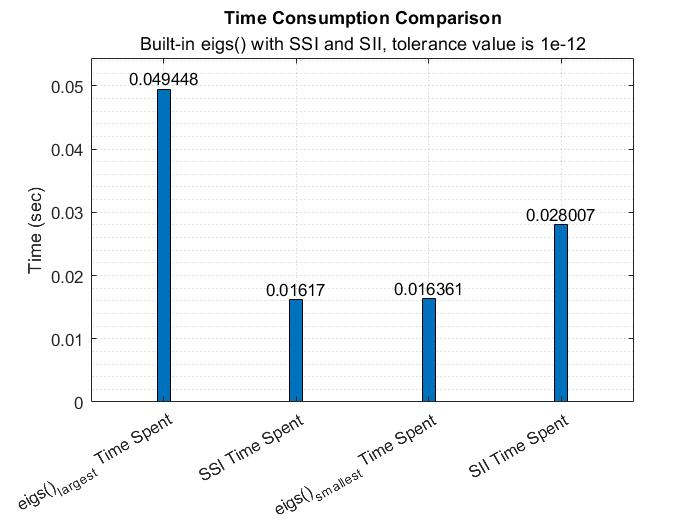
\includegraphics[height=9cm, width=12cm]{plot3bfw.jpg}}
	\caption{\textbf{BFW62B, k = 3} \\ Iteration Number for SSI = 2721, Iteration Number for SII = 3790}
	\label{fig8}
\end{figure}

\begin{figure}[H]
	\centerline{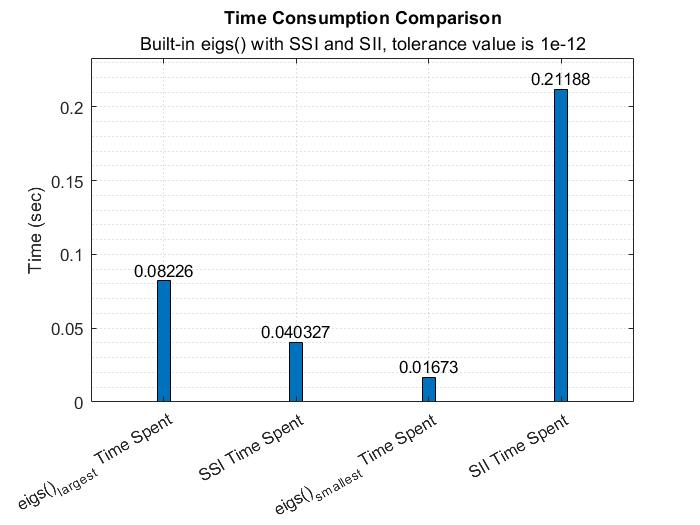
\includegraphics[height=9cm, width=12cm]{plot10bfw.jpg}}
	\caption{\textbf{BFW62B, k = 10} \\ Iteration Number for SSI = 2721, Iteration Number for SII = 11922}
	\label{fig9}
\end{figure}

\begin{figure}[H]
	\centerline{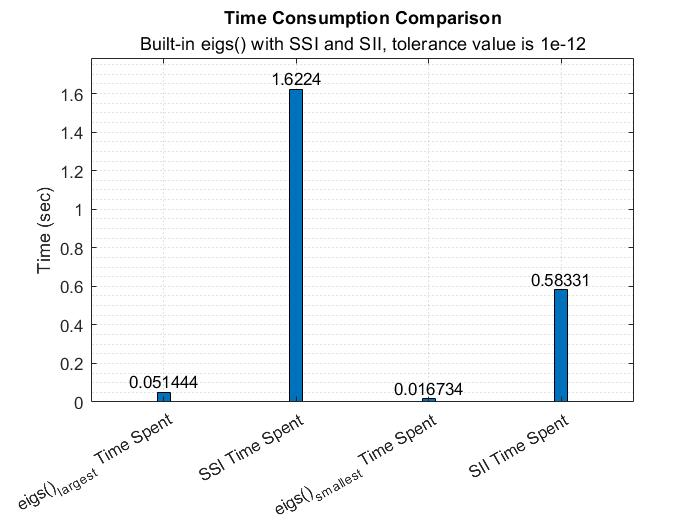
\includegraphics[height=9cm, width=12cm]{plot25bfw.jpg}}
	\caption{\textbf{BFW62B, k = 25} \\ Iteration Number for SSI = 36317, Iteration Number for SII = 11850}
	\label{fig10}
\end{figure}

\begin{figure}[H]
	\centerline{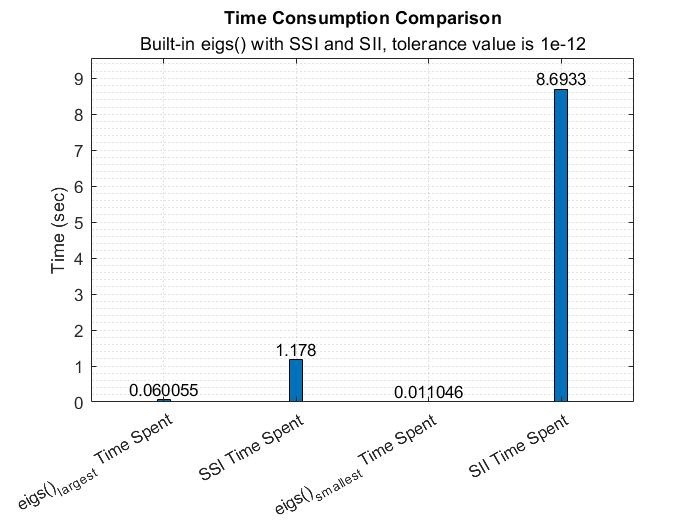
\includegraphics[height=9cm, width=12cm]{plotplat.jpg}}
	\caption{\textbf{PLAT362, k = 1} \\ Iteration Number for SSI \& SII = 100000 (max iterations allowed) \\ PLAT362 coefficient matrix does not converge in implemented methods; however, eigs() function can solve that matrix.}
	\label{fig11}
\end{figure}

\hspace{1cm}


\par \quad SSI is basically finds the largest eigenpairs. Since it always make operations with k-column matrices, the multiplication operation started to take long time as k increases. SII is a mixed method composed of inverse power method, and SSI. It finds the smallest eigenpairs since we take the inverse of the A matrix. Same situation happens for SII. They do not utilize parallelism.
\par \quad MATLAB built-in eigs() function, on the other hand, makes an intense parallelism. It seems that when k=1, implemented SSI and SII even shows better timing performance than eigs() function. As k increases, the effectiveness of parallelism increases. 
\par \quad Proposed method is, we separate each eigenpairs by shifting the original matrix A with different amount. After that, we algorithms work each column independently by different processor units. However, by this way, we can lose some eigen pairs or we can reach the same pairs from different parallel processes.

\pagebreak

\section*{Acknowledgements}
\quad To convert matrices taken from the Matrix Market, "MatrixMarket I/O Functions for Matlab, mmread.m" function is included to the homework codes. \emph{(https://math.nist.gov/MatrixMarket/mmio/matlab/mmiomatlab.html)\\}    
\quad 1st link tells that the eigs() function's parallelism approach., 

\begin{thebibliography}{9}

\bibitem{a}
Parallelism on eigs() function: \\
\emph{https://www.mathworks.com/help/matlab/ref/eigs.html}

\bibitem{b}
Improvement guide to implement proposed method: \\
\emph{https://www.mathworks.com/help/parallel-computing/parallel.gpu.cudakernel.html}

\bibitem{c}
LUND A matrix: \\
\emph{https://math.nist.gov/MatrixMarket/data/Harwell-Boeing/smtape/lund\_a.html}

\bibitem{d}
BFW62B matrix: \\
\emph{https://math.nist.gov/MatrixMarket/data/NEP/bfwave/bfw62b.html}

\bibitem{3}
PLAT362 matrix: \\
\emph{https://math.nist.gov/MatrixMarket/data/Harwell-Boeing/platz/plat362.html}

\end{thebibliography}

\end{document}


